\sec{Deep neural nets (via covering number)}\label{sec:deep_nets}
In Section~\ref{lec9:sec:cover_to_radem}, we discuss how strong our bounds on covering number need to be in order to get a useful result. 
Here we describe some situations in which we know how to obtain these covering number bounds for concrete models such as linear models and neural networks. 

\subsec{Preparation: covering number for linear models}
First, consider the following covering number bound for linear models:

\begin{theorem}[\cite{zhang2002}] \label{lec9:thm:univariate_rad}
Suppose $x^{(1)}, \cdots, x^{(n)} \in \mathbb{R}^d$ are $n$ data points, and $p, q$ satisfies $1/p + 1/q = 1$ and $2 \le p \le \infty$. Assume that $||x^{(i)}||_p \le C$ for all $i$. Let:
\begin{align}
    \cF_q = \{x \mapsto w^\top x : ||w||_q \le B\}
\end{align}
and let $\rho = L_2(P_n)$. Then, $\log N(\epsilon, \cF_q, \rho) \le \l [\frac{B^2C^2}{\epsilon^2}\r ] \log_2 (2d + 1)$. When $p = 2, q = 2$, we further obtain that:
\begin{align}
    \log N(\epsilon, \cF_2, \rho) \le \l [\frac{B^2C^2}{\epsilon^2} \r ] \log_2 (2 \min (n, d ) + 1)
\end{align}
\end{theorem}
\begin{remark}
Applying \eqref{lec9:eqn:rademacherbound_three} to the covering number bound derived above with $R = B^2C^2$, we conclude that the Rademacher complexity of this class of linear models satisfies
\begin{align}
    R_S(\cF_q) &\le \tilO{\left( \frac{BC}{\sqrt{n}} \right)}.
\end{align} 
We also prove this result without relying on Dudley's theorem in Theorem~\ref{lec7:thm:l2-thm}.
\end{remark}
Next, we consider multivariate linear functions as they are building blocks for multi-layer neural networks. Let $M = (M_1, \cdots, M_n) \in \mathbb{R}^{m \times n}$ and $\norm{M}_{2,1} = \sum_{i = 1}^n \norm{M_i}_2$. Then, $\norm{M^\top}_{2,1}$ denotes the sum of the $\ell_2$ norms of the rows of $M$. 
\begin{theorem}\label{lec9:thm:multivariate_rad}
Let $\cF = \{x \to Wx : W \in \mathbb{R}^{m \times d}, ||W^\top||_{2, 1} \le B\}$ and let $C = \sqrt{\frac{1}{n} \sum_{i = 1}^n ||x^{(i)}||_2^2}$. Then, 
\begin{equation}
\log N(\epsilon, \cF, L_2(P_n)) \le \l [\frac{c^2B^2}{\epsilon^2} \r ] \ln (2dm).
\end{equation}
\end{theorem}
\begin{remark}
    In some sense, Theorem~\ref{lec9:thm:multivariate_rad} arises from treating each dimension of the multivariate problem independently. We can view the linear layer as applying $m$ different linear functions. Explicitly, if $W = \begin{pmatrix} w_1^\top \\ \vdots \\ w_m^\top \end{pmatrix}$ and $Wx = \begin{pmatrix} w_1^\top x \\ \vdots \\ w_m^\top x \end{pmatrix}$, then as we expect, $\norm{W^\top}_{2,1} = \sum \norm{w_i}_2$.
\end{remark}


\subsec{Deep neural networks}
In this lecture, we discuss a bound on the Rademacher complexity of a dense neural network. We set up notation as follows: $W_i$ denotes the linear weight matrix at the $i$-th layer of the neural network, we have a total of $r$ layers, and $\sigma$ is the activation function which is 1-Lipschitz (for example, ReLU, softmax, or sigmoid). If the input is a vector $x$, the neural network's output can be represented as follows:

\begin{align}
    f_\theta(x) = W_r\sigma(W_{r-1}\sigma(\cdots \sigma(W_1x)\ldots),
\end{align}
Using this notation, we establish an upper bound on the Rademacher complexity of a dense neural network.

\begin{theorem}[\cite{bartlett2017}]
\label{lec10:thm:dnn_rademacher}
Suppose that $\forall i, \norm{x^{(i)}}_2 \leq c$ and let
\begin{align}
    \cF = \{f_\theta : \norm{W_i}_{\textup{op}} \leq \kappa_i, \norm{W_i^\top}_{2,1} \leq b_i\}.
\end{align}
Then,
\begin{equation}
    R_S (\cF) \leq \frac{c}{\sqrt{n}} \cdot \underbrace{\left(\prod_{i=1}^r \kappa_i \right)}_{\textup{(I)}} \cdot \underbrace{\left( \sum_{i=1}^r\frac{b_i^{2/3}}{\kappa_i^{2/3}}\right)^{3/2}}_{\textup{(II)}}. \label{lec10:eqn:bartlett_rad_bound}
\end{equation}
\end{theorem}
We use $\norm{W}_{\textup{op}}$ to denote the operator norm (or spectral norm) of $W$, and recall that $\norm{W_i^\top}_{2,1}$ denotes the sum of the $\ell_2$ norms of the rows of $W_i$. Examining \eqref{lec10:eqn:bartlett_rad_bound}, we see that (II) is relatively small as it is a sum of matrix norms, and so the bound is dominated by (I), which is a product of matrix norms.

\begin{remark}
    We note that $f(x) = Wx$ is Lipschitz with a Lipschitz constant of $\norm{W}_{\textup{op}}$. This is because 
    \begin{align}
        \norm{f(x)-f(y)}_2 &= \norm{Wx-Wy}_2 \\
        &\leq \norm{W}_{\textup{op}}\norm{x-y}_2 &\text{$(\norm{W}_{\textup{op}} = \max_{x:\norm{x}_2=1}\norm{Wx}_2)$}
    \end{align}. 
\end{remark}

\begin{remark}
    As a corollary of the above theorem, we also get a bound on the generalization error for the margin loss of the following form:
    \begin{equation}
        \textup{generalization error} \leq \tilde{O}\left(\frac{1}{\gamma_{\min}} \cdot \frac{1}{\sqrt{n}} \cdot \left(\prod_{i=1}^r\norm{W_i}_{\textup{op}} \right) \cdot {\left( \sum_{i=1}^r\frac{\norm{W_i^\top}^{2/3}_{2,1}}{\norm{W_i}_{\textup{op}}^{2/3}}\right)^{3/2}}  \right),
    \end{equation}
    where $\gamma_{\min}$ denotes the margin.
\end{remark}
	
First, we motivate the proof by presenting the main idea, and then work through each part of the proof. The main ideas of the proof can be summarized as follows:
    
\begin{itemize}
    \item At a high level, we want to show that the covering number $N(\epsilon, \cF, \rho)$ for a dense neural network is $\leq \frac{R}{\epsilon^2}$. Proving this would enable us to apply Theorem~\ref{lec9:thm:better-dudley} to get a bound on the Rademacher Complexity.
    \item To bound the covering number for a dense neural network, we use $\epsilon$-covers to cover each layer of $f_\theta$ separately, and then combine them to prove that there exists an $\epsilon$-cover of the original function $f_\theta$. 
    \item To combine the $\epsilon$-covers of each layer, we use the Lipschitzness of each layer.
    \item We control and approximate the error propagation that is introduced through discretizing each layer using $\epsilon_i$-coverings in order to get a reasonable final $\epsilon$.
\end{itemize}

As a prelude to the proof of Theorem~\ref{lec10:thm:dnn_rademacher}, let us abstractify each layer of $\cF$ as $\cF_i$ where $\cF_i$ corresponds to matrix multiplication by $W_i$ composed with a nonlinear activation function $\sigma$. We then denote $\cF$ as the composition of each of these (single layer) function spaces as follows:
\begin{align}
    \cF = \cF_r \circ \cF_{r - 1} \circ \cdots \circ \cF_1 = \{f_r \circ f_{r - 1} \circ \cdots f_{1} : f_i \in \cF_i\}
\end{align}
We will assume throughout that $f_i$ is $\kappa_i$-Lipschitz, i.e.
\begin{align}
    \norm{f_i(x) - f_i(y)}_2 \leq \kappa_i \norm{x - y}_2 \label{lec10:eqn:lipschitz-def}
\end{align} 
Let us also assume, for simplicity, that $f_i(0) = 0$ and $\norm{x\sp{j}}_2 \leq c$ for all $j = 1,\dots,n$. Then, by applying the definition of Lipschitz continuity, we obtain that:
\begin{align}
    \norm{f_i(f_{i - 1}(\cdots(f_1(x\sp{j}))))}_2 \leq \underbrace{\kappa_{i} \cdot \kappa_{i - 1} \cdots \kappa_1 \cdot c}_{\defeq c_i}
\end{align}

We now derive an $\epsilon$-covering of $\cF$ in two steps:
\begin{enumerate}
    \item Given inputs to the $i^{th}$ layer, we construct an $\epsilon_i$-covering of the output space of the function $f_i$.
    \item Using the $\epsilon_i$-covering as inputs to the $(i + 1)$-th layer, we show that we can use several single layer coverings to construct an $\epsilon$-covering for a multilayer network.
\end{enumerate}

Formally, the following lemma answers the second step in the above outline. Namely, given a covering number for a single layer, we show how to compute a covering number bound for multiple layers.
\begin{lemma}
    Under the setup given above, if every input to $f_i$ satisfies $\norm{z\sp{j}}_2 \leq c_{i - 1}$, we assume that  
    \begin{align}
        \log N(\epsilon_i, \cF_i, L_2(P_n)) \leq g(\epsilon_i, c_{i - 1}).\footnotemark \label{lec10:eqn:single_cover_bound}
    \end{align}
    \footnotetext{If $\cF_i$ defines a collection of linear models, then $\log N(\epsilon_i, \cF_i, L_2(P_n)) \leq \l \lceil \frac{c_{i - 1}^2}{\epsilon_i^2} \r \rceil$.}
    Then, there exists an $\epsilon$-cover $\cC$ of $\cF_r \circ \cdots \circ \cF_1$ for $\epsilon = \epsilon_r + \kappa_r\epsilon_{r-1} + \cdots + \kappa_r\kappa_{r-1}\dots\kappa_2\epsilon_1$ such that
    \begin{align}
        \log \abs{\cC} \leq \sum_{i=1}^{r} g\left(\epsilon_i, c_{i-1}\right)
    \end{align}
    \label{lec10:lma:additive_cover}
\end{lemma}
\begin{proof}
\tnote{the figure is very important for the proof}
Let $\epsilon_1,\dots,\epsilon_r$ be the radius for each layer. Let $\cC_1$ be an $\epsilon_1$-cover of $\cF_1$. Then, for all $f_1' \in \cC_1$, we define $\cC_{2, f_1'}$ as an $\epsilon_2$-covering of  the set 
\begin{equation}
    \cF_2 \circ f_1' = \left\{f_2\left(f_1'\left(X\right)\right) : f_2 \in \cF_2 \right\}.
\end{equation}
Taking a union of this covering over all $f_1' \in \cC_1$ clearly yields an $\epsilon$-covering for $\cF_2 \circ \cF_2$. In paricular, if 
\begin{align}
    \cC_2 = \bigcup_{f_1'\in \cC_1}\cC_{2,f_1'},
\end{align} 
then $\cC_2$ is an $\epsilon$-cover of $\cF_2 \circ \cF_1$ with $\epsilon = \epsilon_1 \cdot \kappa_2 + \epsilon_2$. We prove this claim rigorously in the sequel.

Next, we bound the sizes of these covers. Directly applying the assumption given by \eqref{lec10:eqn:single_cover_bound}, we conclude that
\begin{align}
    \log \abs{\cC_{2, f_1'}} \leq g\left(\epsilon_2, c_1\right).
\end{align}
Then, because $\cC_2 = \bigcup_{f_1'\in \cC_1}\cC_{2,f_1'}$, it immediately follows that
\begin{align}
    \abs{\cC_{2}} &\leq \abs{\cC_{1}} \exp\left(g\left(\epsilon_2, c_1\right)\right) \label{lec10:eqn:iterative_cover_bound-1}\\
    \log\abs{\cC_{2}} &\leq \log\abs{\cC_{1}} + g\left(\epsilon_2, c_1\right) \\
    &\leq g\left(\epsilon_1, c_0\right) + g\left(\epsilon_2, c_1\right).  \label{lec10:eqn:iterative_cover_bound-3}
\end{align}
Similarly, given $\cC_k$, for any $f_k' \circ f_{k-1}' \circ \cdots \circ f_1' \in \cC_k$, we construct a $\cC_{k+1, f_k', \dots, f_1'}$ that is an $\epsilon_{k+1}$-covering of $\cF_{k+1} \circ f_k' \circ \cdots \circ f_1'$. We similarly define 
\begin{equation}
    \cC_{k+1} = \bigcup_{\substack{f_i \in \cC_i \\ i \leq k}} C_{k+1, f_k', \dots, f_1'}.
\end{equation}
Then, inducting on the argument given in \eqref{lec10:eqn:iterative_cover_bound-1}-\eqref{lec10:eqn:iterative_cover_bound-3}, we conclude that
\begin{align}
    \log \abs{\cC_{k+1}} \leq g\left(\epsilon_{k+1}, c_k\right) + \cdots + g\left(\epsilon_1, c_0\right)
\end{align}
Next, we show that for the above construction, the radius of the cover for $\cF$ is
\begin{align}
    \epsilon = \sum_{i=1}^{r} \left(\epsilon_i \prod_{j=i+1}^{r}\kappa_{j}\right).
\end{align}
For any choice of $f_r \circ \cdots \circ f_1 \in \cF_r \circ \cF_{r-1} \circ \cdots \circ \cF_1$,  then, by definition of $\cC_1$, there exists $f_1' \in \cC_1$ such that 
\begin{equation}
    \rho(f_1, f_1') \leq \epsilon_1.
\end{equation} 
Similarly, we know there exists $f_2' \circ f_1' \in \cC_{2, f_1'}$ such that 
\begin{equation} 
    \rho\left(f_2' \circ f_1', f_2\circ f_1' \right) \leq \epsilon_2.
\end{equation}
We can leverage these two facts and the triangle inequality to now prove that $f_2' \circ f_1'$ is close to $f_2 \circ f_1$. Namely,
\begin{align}
   \rho\left(f_2' \circ f_1', f_2 \circ f_1\right) &\leq \rho\left(f_2' \circ f_1', f_2 \circ f_1'\right) + \rho\left(f_2 \circ f_1', f_2 \circ f_1\right) &\text{(triangle ineq.)} \\ 
   &\leq \epsilon_2 + \rho\left(f_2 \circ f_1', f_2 \circ f_1\right) &\text{(def. of $\cC_{2, f'_1}$)}\\ 
   &\leq \epsilon_2 + \kappa_2 \rho\left(f_1', f_1\right) &\text{\eqref{lec10:eqn:lipschitz-def}}\\ 
   &\leq \epsilon_2 + \kappa_2\epsilon_1 &\text{(def. of $\cC_{1}$)}
\end{align}
Inducting to prove this argument for arbitrary $k$, we similarly apply the definition of $\cC_{k, f'_{k - 1},\dots,f'_1}$ to conclude that there exists $f'_{k} \circ f'_{k - 1} \circ \cdots \circ f'_1 \in \cC_k$ such that
\begin{equation}
    \rho(f'_k \circ f'_{k - 1} \circ \cdots f'_1, f_k \circ f'_{k - 1} \circ \cdots f'_1) \leq \epsilon_k
\end{equation}
Then, expanding using the triangle inequality and peeling off terms by applying the definition of our $\epsilon_i$-coverings, we again show that
\begin{align}
    \rho\left(f_k' \circ f_{k-1}' \circ \cdots \circ f_1', f_k \circ \cdots \circ f_1\right) &\leq \rho\left(f_k' \circ f_{k-1}'\circ \cdots \circ f_1', f_k \circ f_{k-1}'\circ \cdots \circ f_1' \right) \\ 
    &\quad + \rho\left(f_k \circ f_{k-1}'\circ f_{k-2}' \circ \cdots \circ f_1', f_k \circ f_{k-1}\circ f_{k-2}' \circ \cdots \circ f_1'\right) \nonumber \\ 
    &\quad + \cdots + \rho\left(f_k \circ f_{k-1}\circ \cdots \circ f_2 \circ f_1', f_k \circ f_{k-1}\circ \cdots \circ f_1\right) \nonumber \\ 
    &\leq \rho\left(f_k' \circ f_{k-1}'\circ \cdots \circ f_1', f_k \circ f_{k-1}'\circ \cdots \circ f_1' \right) \\
    &\quad + \kappa_{k} \cdot \rho(f'_{k - 1} \circ \cdots \circ f'_1, f_{k - 1} \circ f'_{k - 2} \circ \cdots \circ f'_1) \\
    &\quad + \cdots + \left(\prod_{j = 2}^k \kappa_j\right) \rho(f'_1, f_1) \nonumber  \\
    & \leq \sum_{i=1}^{k} \left(\epsilon_i\prod_{j=i+1}^{k}\kappa_{j}\right).
\end{align}
Note that the first inequality follows by the triangle inequality, the second by the $\kappa_i$-Lipschitz continuity of $f_i$, and the third by applying the definition of each of our $\epsilon_i$-covers.
\end{proof}

\begin{proof}[Proof of Theorem~\ref{lec10:thm:dnn_rademacher}]
We now apply Lemma~\ref{lec10:lma:additive_cover} to dense neural networks. Dense neural networks consist of a composition of layers, where each layer is a linear model composed with a 1-Lipschitz activation. Using Theorem~\ref{lec9:thm:multivariate_rad} along with the property that 1-Lipschitz functions will only contribute a factor of at most $1$ (Lemma~\ref{lec9:lma:talagrand}), the covering number of each layer can be bounded by:
\begin{align}
    g\left(\epsilon_i, c_{i-1}\right) = \tilde{O}\left(\frac{c_{i-1}^2b_i^2}{\epsilon_i^2}\right),
\end{align}
where $c_{i-1}^2$ is the norm of the inputs, $b_i^2$ is $\norm{W_i^\top}_{2,1}$, and $\epsilon_i^2$ is the radius. From Lemma~\ref{lec10:lma:additive_cover}, we know that 
\begin{align}
    \log N(\epsilon, \cF, \rho) &= \tilde{O}\left(\sum_{i=1}^{r}\frac{c_{i-1}^2b_i^2}{\epsilon_i^2}\right) 
\end{align}
for
\begin{align}
    \epsilon &= \sum_{i=1}^{r} \left(\epsilon_i \prod_{j=i+1}^{r}\kappa_j\right)
\end{align}

We now have a bound on $N(\epsilon, \cF, \rho)$ that relies on $\epsilon_i$'s, but $N(\epsilon, \cF, \rho)$ should only be a function of $\epsilon$. Since we already know that $\epsilon = \sum_{i=1}^{r} \left(\epsilon_i \prod_{j=i+1}^{r}\kappa_j\right)$, we keep $\epsilon$ constant and optimize the upper bound of $N(\epsilon, \cF, \rho)$ over different choices of $\epsilon_i$. To find the optimal $\epsilon_i$, we will first find a lower bound on $N(\epsilon, \cF, \rho)$. We then choose $\epsilon_i$ so that this lower bound is achieved. Ultimately, our optimized $\epsilon_i$ yields a bound on the covering number of the following form: $\log\left(N\left(\epsilon, \cF, \rho\right)\right) \leq \frac{R}{\epsilon^2}$, where $R$ is some constant independent of $\epsilon$. 

We derive this lower bound using Holder's inequality, which states that
\begin{align}
    \langle a,  b \rangle \leq \|a\|_p \|b\|_q
\end{align}
when $\frac{1}{p} + \frac{1}{q} = 1$. Writing out the vectors $a, b$, we get that 
\begin{align}
    \sum_{i}a_ib_i \leq \left(\sum a_i^p\right)^{\frac{1}{p}}\left(\sum b_i^q\right)^{\frac{1}{q}}
\end{align}

Letting $\alpha_i^2 = c_{i-1}^2b_i^2, \beta_i = \prod_{j=i+1}^{r}\kappa_j$. By Holder's inequality, using $p = 3, q = \frac{3}{2}$, we get
\begin{align}
    \left(\sum_{i=1}^{r}\frac{\alpha_i^2}{\epsilon_i^2}\right)\left(\sum_{i=1}^{r}\beta_i\epsilon_i\right)^2 &\geq \left(\sum_{i=1}^{r}\left(\alpha_i\beta_i\right)^{\frac{2}{3}}\right)^{\frac{3}{2}}
\end{align}
\begin{align}
    \sum_{i=1}^{r}\frac{\alpha_i^2}{\epsilon_i^2} &\geq \frac{R}{\epsilon^2},
\end{align}
where $R = \left(\left(\sum_{i=1}^{r}\left(c_{i-1}b_i\prod_{j=i+1}^{r}\kappa_j\right)\right)^{\frac{2}{3}}\right)^{\frac{3}{2}}$. We note that equality holds when 
\begin{align}
    \epsilon_i = \left(\frac{c_{i-1}^2b_i^2}{\prod_{j=i+1}^{r}\kappa_j}\right)^{\frac{1}{3}} \cdot \underbrace{\frac{\epsilon}{\left(\sum_{i=1}^{r}\frac{b_i^{\frac{2}{3}}}{\kappa_i^{\frac{2}{3}}}\right)\prod_{i=1}^{r}\kappa_i^{\frac{2}{3}} }}_{\epsilon'} \label{eqn:lec10:holder_eps_defn}
\end{align}
Using this choice of $\epsilon_i$ and letting $\epsilon'$ equal the second factor in \eqref{eqn:lec10:holder_eps_defn} for notational convenience, we know that the log covering number is (up to a constant factor):
\al{
    \sum_{i=1}^r \frac{c_{i-1}^2b_i^2}{\epsilon_i^2} &= \sum_{i=1}^r \frac{c_{i-1}^2b_i^2(\kappa_{i+1}\cdots\kappa_r)^\frac{2}{3}}{c_{i-1}^\frac{4}{3}b_i^\frac{4}{3}(\epsilon')^2} \\
    &= \sum_{i=1}^r (c_{i-1}b_i\kappa_{i+1}\cdots\kappa_r)^\frac{2}{3}\frac{1}{(\epsilon')^2} \\
    &= c^\frac{2}{3}\sum_{i=1}^r \left(\frac{b_i}{\kappa_i}\right)^\frac{2}{3} \prod_{i=1}^r \kappa_i^\frac{2}{3} \frac{\left(c^\frac{2}{3}\left(\sum_{i=1}^r (\frac{b_i}{\kappa_i})^\frac{2}{3} \prod_{i=1}^r \kappa_i^\frac{2}{3}\right)\right)^2}{\epsilon^2} \\
    &= \left(c^\frac{2}{3}\sum_{i=1}^r \left(\frac{b_i}{\kappa_i}\right)^\frac{2}{3} \prod_{i=1}^r \kappa_i^\frac{2}{3}\right)^3\frac{1}{\epsilon^2} \\
    &= c^2\prod_{i=1}^r \kappa_i^2\left(\sum_{i=1}^r \left(\frac{b_i}{\kappa_i}\right)^\frac{2}{3}\right)^3\frac{1}{\epsilon^2}.
}
Since this log covering number is of the form $R / \epsilon^2$, we can apply \eqref{lec9:eqn:rademacherbound_three} and conclude that
\al{
    \mathcal{R}_S(\cF) \lesssim \sqrt\frac{R}{n}
}
Last, plugging in
\al{
    R = c^2\prod_{i=1}^r \kappa_i^2\left(\sum_{i=1}^r \left(\frac{b_i}{\kappa_i}\right)^\frac{2}{3}\right)^3
}
we obtain the desired result
\al{
    \mathcal{R}_S(\cF) \lesssim \frac{c}{\sqrt n}\prod_{i=1}^r \kappa_i\left(\sum_{i=1}^r \left(\frac{b_i}{\kappa_i}\right)^\frac{2}{3}\right)^\frac{3}{2}.
}

\end{proof}

\chapter{Data-dependent Generalization Bounds for Deep Nets}\label{sec:deep_nets_data_dependent}

In Theorem~\ref{lec10:thm:dnn_rademacher}, we proved the following bound on the Rademacher complexity of deep neural networks:
\begin{align}
    R_S(\cF) \leq \prod_{i = 1}^r \norm{W_i}_{\text{op}} \cdot \mathsf{poly}(\norm{W_1}, \dots, \norm{W_r}).
\end{align}
This bound, however, suffers from multiple deficiencies. In particular, it grows exponentially in the depth, $r$, of the network and $\norm{W_i}_{\text{op}}$ measures the worst-case Lipschitz-ness of the network layers over the input space. %As a consequence, the bound fails to accurately predict the good generalization properties of deep nets.

In this section, we obtain a tighter generalization bound that depends upon the realized Lipschitz-ness of the model on the training data. To further motivate this approach, we also note that stochastic gradient descent, i.e. the typical optimization method typically used to fit deep neural networks, prefers models that are more Lipschitz (see Chapter (TBD) for further discussion) \tnotelong{add references later}. This preference must be realized by the model \emph{on empirical data}, however, as no learning algorithm has access to the model's properties over the entire data space.

Ultimately, we aim to prove a tighter bound on the population loss that grows polynomially in the Lipschitz-ness of $f$ on the empirical data. Namely, given that $f$ is parameterized by some $\theta$, we hope to derive a bound on the population loss at $\theta$ that is a \emph{polynomial} function of the Lipschitz-ness of $f$ on $x\sp{1},\dots,x\sp{n}$ as well as the norm of $\theta$.

\paragraph{Uniform convergence with a data-dependent hypothesis class.}
%Classical uniform convergence does not have a single consistent definition. 
So far in this course, given some complexity measure we denote as $\text{comp}(\cdot)$, our uniform convergence results always appear in one of the two following forms (which are essentially equivalent). Namely, with high probability,
\begin{align}
\forall f\in \cF, ~~L(f) &\leq \frac{\text{comp}(\cF)}{\sqrt{n}} &&\text{(I)} \\
\forall f, ~~ L(f) &\leq \frac{\text{comp}(f)}{\sqrt{n}}  &&\text{(II)}
\end{align}

\begin{remark}
    Most of the results we have obtained so far are of type I, e.g. with $\text{comp}(\cF)/\sqrt{n} = R_n(\cF)$. We obtain results of type II by considering a restricted set of functions $\cF_C = \{f : \text{comp}(f) \leq C\}$. We then apply a type I bound to $\cF_C$ and take a union bound over all $C$. Therefore, these two type of bounds are essentially equivalent (up to a small additive factor difference due to the additional union bound over the choices of $C$.)
\end{remark}

Note, however, that neither of these approaches produce bounds that depend upon the data. By contrast, in the sequel, we will derive a new \textit{data-dependent} generalization bound. These bounds state that with high probability over the choice of the empirical data and, for all functions $f\in \cF$,
\begin{align}
    L(f) \leq \text{comp}\left (f, \{(x\sp{i}, y\sp{i})\}_{i = 1}^n\right)
\end{align}
Even though the complexity measure depends on the training data, and is thus a random variable by itself, it can be used as a regularizer which can be added to the original training loss.

\begin{remark}
Although there is no universal consensus on the type of generalization bound we should derive, we can argue that there is no way to leverage more information in a generalization bound beyond the empirical data. For example, one might try to use the input distribution $P$ to define the complexity measure, but if we allowed ourselves access to $P$, we could just define $\text{comp}(f, P) = \Exp_P[f(X)]$. In some sense, defining a generalization bound using the true distribution amounts to cheating, and the dependence on the empirical data seems to be proper because the bound can still be used as a regularizer. %, so it becomes difficult to define a distibution-dependent generalization bound in a principled way.
\end{remark}

In this new paradigm, we can no longer take the previous approach of obtaining type I bounds and then derive a type II bound via a reduction. To see why, suppose that we have the hypothesis class
\begin{align}
    \cF_C = \{f: \text{comp}(f, \{(x\sp{i}, y\sp{i})\}_{i=1}^n) \leq C)\}
\end{align}
If our complexity measure depends on the empirical data, then so does our hypothesis class $\cF_C$, which makes $\cF_C$ itself a random variable. However, our theorems regarding Rademacher complexity require that the hypothesis class be fixed before we ever see the empirical data.

We may hope to get around this by changing the way we think about uniform convergence. Consider the simplified case where our new complexity measure is separable, i.e.
\begin{align}
    \text{comp}(f, \{(x\sp{i}, y\sp{i})\}_{i=1}^n) = \sum_{i=1}^n h(f, x\sp{i}),
\end{align}
for some function $g$. Then we can consider an \textit{augmented loss}:
\begin{align}
    \tilde{\ell}(f) = \ell(f) \ind{h(f, x\sp{i} \leq C)} \label{eqn:5}
\end{align}
\begin{figure}[ht]
    \centering
    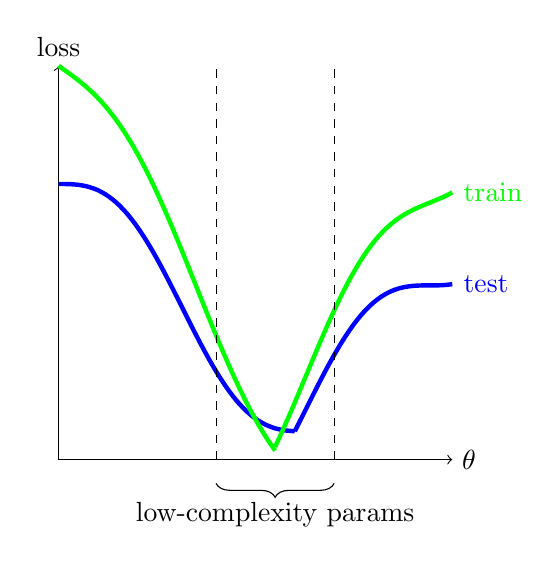
\begin{tikzpicture}
        \draw[->] (0, 0) -- (5, 0) node[right] {$\theta$};
        \draw[->] (0, 0) -- (0, 5) node[above] {loss};
        \draw[scale=0.5, domain=0:6, smooth, ultra thick, variable=\x, blue] plot (\x, {7 - \x + sin(\x r)});
        \draw[scale=0.5, domain=0:5.5, smooth, ultra thick, variable=\x, green] plot (\x, {10 - 1.6*\x + sin(0.90*\x r)});
        \draw[scale=0.5, domain=6:10, smooth, ultra thick, variable=\x, blue] plot (\x, {\x - 5 + sin(\x r)}) node[right] {test};
        \draw[scale=0.5, domain=5.5:10, smooth, ultra thick, variable=\x, green] plot (\x, {1.4*\x - 6.67 + sin(\x r)}) node[right] {train};
        \draw[dashed] (2, 0) -- (2, 5);
        \draw[dashed] (3.5, 0) -- (3.5, 5);
        \draw [decorate,decoration={brace,amplitude=5pt,mirror,raise=2ex}]
        (2,0) -- (3.5,0) node[midway,yshift=-2em]{low-complexity params};
    \end{tikzpicture}
    \caption{These curves depict a ``low-complexity'' region in parameter space. The \textcolor{blue}{blue} curve is the unobserved test loss we aim to bound, while the \textcolor{green}{green} curve denotes the empirical training loss we observe. Observe that in the region of $\theta$ that we identify as being ``low-complexity,'' the gap between the train and test losses is smaller than in the high-complexity regions.}
    \label{lec11:fig:low_vs_high_complexity}
\end{figure}
Suppose we have a region of low complexity in our existing loss function as depicted in Figure~\ref{lec11:fig:low_vs_high_complexity}. Because this region is random, so we cannot selectively apply uniform convergence. However, we can use our new surrogate loss function $\tilde{\ell}$ in that region. By modifying the loss function in this way, we can still fix the hypothesis class ahead of time, allowing us to apply existing tools to $\tilde{\ell}(f)$. The surrogate loss was used in~\cite{wei2019data} to obtain a data-dependent generalization bound, though there are possibly various other ways to define surrogate losses and apply existing uniform convergence guarantees. In the sequel, we introduce a particular surrogate ``margin'' that allows us to cleanly apply our previous results to a (implicitly) data-dependent hypothesis class \cite{wei2019data}.

\sec{All-layer margin} \label{sec:all_layer_margin}
We next introduce a new surrogate loss called the \textit{all-layer margin} that can also be thought of as a surrogate margin. This loss will essentially zero out high-complexity regions so that we may focus on low-complexity regions for which we can expect small generalization gap. Note that the all-layer margin we analyze will not explicitly zero-out high-complexity regions using an indicator function, but instead implicitly takes into account some data-dependent characteristics of the model. Once we adopt this new loss function, we will be able to apply some of our earlier methods.

Let $f: \R^d \to \R$ be a classification model. Recall that the standard margin is defined as $y f(x)$, with $y$ in $\{-1, 1\}$. We will say that $g_f(x, y)$ is a \textit{generalized margin} if it satisfies
\begin{align}
    g_f(x, y) = \begin{cases}
0,& \text{ if } f(x)y \leq 0 \text{ (an incorrect classification)}\\
> 0,& \text{ if } f(x)y > 0 \text{ (a correct classification)}
\end{cases}.
\end{align}
%That is, the generalized margin ``zeroes out" incorrect classifications.
To simplify the exposition of the machinery below, we also introduce the \textit{$\infty$-covering number} $N_\infty(\epsilon, \cF)$ as the minimum cover size with respect to the metric $\rho$ which is the infinity-norm distance on an input domain $\cX$: 
\begin{equation}
\rho(f, f) \triangleq \sup_{x \in \mathcal{X}} |f(x) - f'(x)| \triangleq \|f - f'\|_\infty.\footnote{If $f$ maps $\cX$ to multi-dimensional outputs, we will define $\rho(f, f) \triangleq \sup_{x \in \mathcal{X}} \|f(x) - f'(x)\| \triangleq \|f - f'\|_\infty$ where the norm in $\|f(x) - f'(x)\|$ is a norm in the output space of $f$ (which will be the Euclidean norm in this rest of this section).}
\end{equation}
\begin{remark}
    Notice that $N_\infty(\epsilon, \cF) \geq N(\epsilon, \cF, L_2(P_n))$. This is because the $\rho = L_\infty(\cX)$ is a more demanding measure of error: $f$ and $f'$ must be close on \textit{every} input, not just the empirical data. That is,
    \begin{equation}
    \sqrt{\frac{1}{n} \sum_{i=1}^n (f(x_i) - f'(x_i))^2} \leq \sup_{x \in \mathcal{X}} |f(x) - f'(x)|. \label{lec11:eqn:l_inf_vs_l2pn}
    \end{equation}
\end{remark}

\begin{lemma}
Suppose $g_f$ is a generalized margin. Let $\cG = \{g_f: f \in \mathcal{F}\}$. Suppose that for some $R$, $\log N_\infty(\epsilon, \cG) \leq \lfloor \frac{R^2}{\epsilon^2} \rfloor$ for all $\epsilon > 0$.\footnote{Recall that this is the worst dependency on $\epsilon$ that we can tolerate when converting covering number bounds to Rademacher complexity.} Then, with probability greater than or equal to $1 - \delta$ over the randomness in the training data, for every $f$ in $\mathcal{F}$ that correctly predicts all the training examples,
\begin{equation}
L_{01} \leq \tilO \l (\frac{1}{\sqrt{n}} \cdot \frac{R}{\min_{i \in [n]} g_f(x\sp{i}, y\sp{i})} \r ) + \tilO\l (\frac{1}{\sqrt{n}}\r ).
\end{equation}
\label{lec11:genmargin-lemma}
\end{lemma}

\begin{proof}
The high-level idea of our proof is to replace $\cF$ with $\cG$ before repeating the standard margin theory argument from Section~\ref{sec:formal_margin}.

Let $\ell_\gamma$ be the ramp loss given in \eqref{lec6:eqn:ramp_loss}, which is 1 for negative values, 0 for values greater than $\gamma$, and a linear interpolation between 1 and 0 for values between 0 and $\gamma$. 
We define the surrogate loss as $\hat{L}_\gamma(\theta) = \frac{1}{n} \sum_{i = 1}^n \ell_\gamma(g_{f_\theta}(x\sp{i}, y\sp{i}))$, and the surrogate population loss as $L_\gamma(\theta) = \Exp[\ell_\gamma(g_{f_\theta}(x, y))]$. Applying Corollary~\ref{lec6:cor:ggap-rsbound}, where we used the Rademacher complexity to control the generalization error, we conclude that
\begin{equation}
L_\gamma(\theta) - \hat{L}_\gamma(\theta) \leq R_S(\ell_\gamma \circ \cG) + \tilO\l (\frac{1}{\sqrt{n}}\r ).
\end{equation}
Next we observe that 
\begin{align}
    \log N(\epsilon, \ell_\gamma \circ \cG, L_2(P_n)) &\leq \log N(\epsilon\gamma, \cG, L_2(P_n)) &\text{(Lemma~\ref{lec9:lma:talagrand})} \\
    &\leq \log N_\infty(\epsilon\gamma, \cG) &\text{\eqref{lec11:eqn:l_inf_vs_l2pn}} \\
    &\leq \l \lfloor \frac{R^2}{\epsilon^2 \gamma^2} \r \rfloor &\text{(by assumption)}.
\end{align}
Then, using our results relating the log of the covering number to a bound on the Rademacher complexity (recall \eqref{lec9:eqn:rademacherbound_three} and Theorem~\ref{lec9:thm:better-dudley}), we conclude that $R_S(\ell_\gamma \circ \cG) \leq \tilO\l (\frac{R}{\gamma \sqrt{n}}\r )$.
Take $\gamma = \gamma_{\min} = \min_{i} g_\gamma(x\sp{i}, y\sp{i})$.\footnote{A caveat: because $\gamma$ is a random variable, proving this result rigorously requires taking a union bound over a discretized $\gamma$. We sketched out this argument more thoroughly in Remark~\ref{lec7:rmk:union_bound_margin}.} Using Corollary~\ref{lec6:cor:ggap-rsbound}, we conclude that $\hat{L}_{\gamma_\text{min}} (\theta) \leq 0 + \tilO\l (\frac{R}{\sqrt{n} \cdot \gamma_\text{min}} \r ) + \tilO\l (\frac{1}{\sqrt{n}}\r )$, as desired.
\end{proof}
For which $g_f$ can we bound the covering number? If we take $g_f(x, y) = yf(x)$, then the covering number depends on the product $\prod_i \norm{W_i}_{\text{op}}$, but we originally set out to do better than this. If we have a linear model $w^\top x$, the normalized margin, $\frac{y \cdot w^\top x}{\norm{w}}$, governs the generalization performance. But how do we normalize for more general models? 

For a deep neural net, a natural normalizer is the product of the Lipschitz constants of the layers. However, we do not want to normalize by a constant that depends only on the function class, so we take a different approach. We interpret the normalized margin as the solution to the following optimization problem:
\begin{equation}
    \begin{aligned}
        \min_\delta \quad & \norm{\delta}_2 \\
        \textrm{s.t.} \quad & w^\top(x + \delta) y \leq 0
    \end{aligned}
\end{equation}
In plain English, how can we find the minimum perturbation that gets our data point across the boundary?

This perturbation view of the standard margin can be extended naturally to multiple layers, but it turns out that mathematically we need to perturb all the layers. We define the \textit{all-layer margin} as below. We will consider perturbed models $\delta = (\delta_1, \dots, \delta_r)$, where each $\delta_i$ is a perturbation \textit{vector} associated with the $i$-th layer (and it has the same dimensionality as the $i$-th layer activation). We incorporate these perturbations into our model in the following particular way (so that we can handle the scaling in a clean way):
\begin{align}
    h_1(x, \delta) &= W_1 x + \delta_1 \cdot \norm{x}_2 \\
    h_2(x, \delta) &= \sigma(W_2 h_1(x, \delta)) + \delta_2 \cdot \norm{h_1(x, \delta)}_2 \\
    &\vdots \nonumber \\
    f(x, \delta) = h_r(x, \delta) &= \sigma(W_r h_{r - 1}(x, \delta)) + \delta_r \cdot \norm{h_{r - 1}(x, \delta)}_2.
\end{align}
We can then ask: what was the smallest perturbation that changed our decision? That is, let
\begin{align}
    m_f(x, y) \defeq \min_\delta \sqrt{\sum_{i=1}^r ||\delta_i||_2^2} \quad \text{s.t.} \quad f(x, \delta) y \leq 0,
\end{align}
i.e. the perturbation yields incorrect predictions.

Informally, $m_f(x, y)$ is a measure of how hard it is to perturb the model $f$. $f$ can be hard to perturb for two reasons: $f$ is Lipschitz (in its intermediate layers) and/or $yf(x)$ is large. In other words, the all-layer margin is a normalized version of the standard margin, normalized by the Lipschitzness of the model at the particular data point $(x,y)$.  %Even more informally, large margins imply confidence in our predictions, and so it becomes harder to change the model's mind.

We now introduce our main result regarding the all-layer margin.
\begin{theorem} \label{lec11:thm:poly_gen_bound_deep_nets}
With high probability,
\begin{equation}
L_{01}(f) \leq \tilO\l (\frac{1}{\sqrt{n}} \cdot \frac{\sum_{i=1}^r \norm{W_i}_{1, 1}}{\min_{i \in [n]} m_f(x\sp{i}, y\sp{i})}\r ) + \tilO\l (\frac{r}{\sqrt{n}}\r ),
\end{equation}
where
$\norm{W}_{1, 1}$ is the sum of the absolute values of the entries of W.
\end{theorem}
In summary, robustness to perturbations in intermediate layers implies good generalization. We will interpret the bound, compare the bounds with previous works, and discuss further extensions in the remarks following the proofs of the theorem.  (E.g, in Remark~\ref{remark:1}, we will argue that this bound is strictly better than the one we obtained in Theorem~\ref{lec10:thm:dnn_rademacher}; in the worst case, we still have that $\frac{1}{m_f(x, y)} \leq \frac{\prod \norm{W_i}_{\text{op}}}{f(x)}$.)

To prove this theorem, it suffices to bound $N_\infty(\epsilon, \cG)$ by $O(\frac{\sum{\norm{W_i}_{1, 1}}}{\epsilon^2})$ and apply Lemma~\ref{lec11:genmargin-lemma}. Towards this goal, let $\cF_i = \{ z \mapsto \sigma (W_i z) : \norm{W_i}_{1, 1} \leq \beta_i \}$. Then, $\cF = \cF_r \circ \cF_{r-1} \circ \cdots \circ \cF_1$. 

\begin{lemma}[Decomposition Lemma]\label{lec11:lma:decomp}
Let $m \circ \cF$ denote $\{m_f : f \in \cF \}$. Then, 
\begin{equation}
\log N_\infty\l (\sqrt{\sum_{i=1}^r \epsilon_i^2}, m \circ \cF \r ) \leq \sum_{i=1}^r \log N_\infty(\epsilon_i, \cF_i),
\end{equation}
where $N_\infty(\epsilon_i, \cF_i)$ is defined with respect to the input domain $\mathcal{X} = \{x : \norm{x}_2 \leq 1 \}$.
\end{lemma}

That is, we only have to find the covering number for each layer, and then we have the covering number for the (all-layer margin of the) composed function class. Notice that we bounded the covering number of $m \circ \cF$ in the above lemma, not $\cF$.

Then, the desired result follows directly from the preceding decomposition lemma.
\begin{corollary} Assume that $\log N_\infty(\epsilon_i, \cF_i) \leq \l \lfloor \frac{c_i^2}{\epsilon_i^2} \r \rfloor$ for every $\cF_i$, i.e. the function class corresponding to the $i$-th layer of $f$ in Theorem~\ref{lec11:thm:poly_gen_bound_deep_nets}. Then, by taking $\epsilon_i = \epsilon \cdot \frac{c_i}{\sqrt{\sum_i c_i^2}}$, we have that
\begin{equation}
    \log N_\infty(\epsilon, m \circ \cF) \leq \frac{\sum_i c_i^2}{\epsilon^2}.
\end{equation}
\end{corollary}
This result gives the complexity of the composed model in terms of the complexity of the layers, with each $c_i$ given by $\norm{W_i}_{1, 1}$. For linear models, we can show $N_\infty(\epsilon_i, \cF_i) \leq \tilO\l (\frac{\beta_i^2}{\epsilon^2} \r )$ (where $\beta_i$ is a bound on $\norm{W_i}_{1, 1}$), and this implies Theorem~\ref{lec11:thm:poly_gen_bound_deep_nets}. Finally, we are only left with the proof of Lemma~\ref{lec11:lma:decomp}. 

\begin{proof}[Proof of Lemma~\ref{lec11:lma:decomp}]
Now we will prove a limited form of the decomposition lemma for affine models: $\cF_i = \{ z \mapsto \sigma(W_i z): \norm{W_i}_{1, 1} \leq \beta_i \}$. There are two crucial steps to this problem. First, we will prove that $m_f(x, y)$ is 1-Lipschitz in $f$. That is, for all $\cF = \cF_r \circ \cF_{r-1} \circ \cdots \circ \cF_1$ and $\cF' = \cF_r' \circ 
\cF_{r-1}' \circ \cdots \circ \cF_1'$,
\begin{align}
    \abs{m_f(x, y) - m_{f'}(x, y)} \leq \sqrt{\sum_{i=1}^r \max_{\norm{x}_2 \leq 1} \norm{f_i(x) - f_i'(x)}_2}. \label{lec11:eqn:one_lipschitz_claim}
\end{align}
Notice that now we are working with a clean sum of differences, with no multipliers! 

Second, we construct a cover: Let $U_1, \dots, U_r$ be $\epsilon_1, \dots, \epsilon_r$-covers of $\cF_1, \dots, \cF_r$, respectively, such that $\abs{U_i} = N_\infty(\epsilon_i, \cF_i)$. By definition, for all $f_i$ in $\cF_i$, there exists a $u_i \in U_i$ such that $\max_{\norm{x} \leq 1} \norm{f_i(x) - u_i(x)}_2 \leq \epsilon_i$. Take $U = U_r \circ U_{r-1} \circ \cdots \circ U_1 = \{u_r \circ u_{r-1} \circ \cdots \circ u_1 \}$ as the cover for $m \circ \cF$. Suppose we were given $f = f_r \circ \cdots \circ f_1 \in \cF$. Let $u_r, \dots, u_1$ be the nearest neighbors of $f_r, \dots, f_1$. Then
\begin{align}
|m_f(x, y) - m_u(x, y)| &\leq \sqrt{\sum_{i=1}^r \max_{||x|| \leq 1} ||f_i(x) - u_i(x)||_2^2} \\
&\leq \sqrt{\sum_{i=1}^r \epsilon_i^2} &&\text{(by construction).}
\end{align}

Having established the validity of our cover, we now return to our claim of 1-Lipschitz-ness stated in \eqref{lec11:eqn:one_lipschitz_claim}. By symmetry, it is sufficient to prove an upper bound for $m_{f'}(x, y) - m_f(x, y)$.

Let $\delta_1^*, \dots, \delta_r^*$ be the optimal choices of $\delta$ in defining $m_f(x, y)$. Our goal is to turn these into a feasible solution of $m_{f'}(x, y)$, which we denote by $\hat{\delta}_1, \dots, \hat{\delta}_r$. In particular, we have that $m_{f'}(x, y) \leq \sqrt{\sigma \norm{\hat{\delta}_i}_2} \leftrightarrow \sqrt{\sigma||\delta_i||^2}$; the solution must be feasible for this bound on $m_{f'}(x, y)$ to hold.

Intuitively, we want to define a perturbation for $f'$ that does the same thing as $\delta_1^*,\dots,\delta_r^*$ for $f$. In plain English, $(f', \hat{\delta}_1, \dots, \hat{\delta}_r)$ should do the same thing as $(f_1, \delta_1^*, \dots, \delta_r^*)$. Recall that $f$ has parameters $W_1, \dots, W_r$ and $f'$ has parameters $W_1', \dots, W_r'$. Then, under the optimal perturbation,
\begin{align}
    h_1 &= W_1 x + \delta_1^* \norm{x}_2 \\
    h_2 &= \sigma(W_2 h_1) + \delta_2^* \norm{h_1}_2 \\
    &\vdots \nonumber \\
    h_r &= \sigma(W_r h_{r - 1}) + \delta_r^* \norm{h_{r - 1}}_2
\end{align}
We want to imitate this by perturbing $f'$ in some way. In particular, let
\begin{equation}
    h_1 = W_1'x + \underbrace{\delta_1^* \norm{x}_2 + (W_1 - W_1')x}_{\defeq \text{ }\hat{\delta}_1 \norm{x}_2},
\end{equation}
where the last term serves to compensate for the difference between $W_1$ and $W_1'$. Thus, $\hat{\delta}_1 \defeq \delta_1^* + \frac{(W_1 - W_1')x}{\norm{x}_2}$.
We repeat this argument for every layer. Using the second layer as an example, 
\begin{align}
    h_2 &= \sigma(W_2' h_1) + \underbrace{\delta_2^*\norm{h_1} + \sigma(W_2 h_1) - \sigma(W_2' h_1)}_{\defeq \text{ }\hat{\delta}_2 \norm{h}_2}.
\end{align}
So, $\hat{\delta}_2 = \delta_2^* + \frac{\sigma(W_2 h_1) - \sigma(W_2' h_1)}{\norm{h_1}_2}$. In general, 
\begin{align}
    \hat{\delta}_i \defeq \delta_i^* + \frac{\sigma(W_ih_{i-1}) - \sigma(W_i' h_{i-1})}{\norm{h_{i-1}}_2}
\end{align} 

Then $\hat{\delta}_1,\dots, \hat{\delta}_r$ on $f'$ are making the same predictions as $\delta_1, \dots, \delta_r$ on $f'$. Last, observe that
\begin{align}
    m_{f'}(x, y) &\leq \sqrt{\sum ||\hat{\delta}_i||_2^2} \\
    &\leq \sqrt{\sum \norm{\delta_i^*}_2^2} + \sqrt{\sum_{i = 1}^r \left (\frac{\sigma(W_i h_{i-1}) - \sigma(W_i' h_{i-1})}{\norm{h_{i-1}}_2} \right)^2 } &\text{(Minkowski's Ineq.)\footnotemark}\\
    &\leq m_f(x, y) + \sqrt{\sum_{i=1}^r \max_{\norm{x}_2 \leq 1} (\sigma(W_i x)-\sigma(W'_i x))^2} \label{lec11:eqn:l2_constraint} \\
    &= m_f(x, y) + \sqrt{\sum_{i=1}^r \max_{\norm{x}_2 \leq 1} (f_i(x)-f_i'(x))^2}
\end{align} 
\footnotetext{Minkowski's inequality, which states that $\sqrt{\sum \norm{a_i + b_i}_2^2} \leq \sqrt{\sum \norm{a_i}_2^2} + \sqrt{\sum \norm{b_i}_2^2}$. In this setting, this inequality can also be proved using Cauchy-Schwarz.}
Note that in \eqref{lec11:eqn:l2_constraint}, constraining $\norm{x}_2 \leq 1$ is equivalent to dividing by the $\ell_2$-norm of $x$.
\end{proof}

\begin{remark}\label{remark:1}
We can compare the above with Theorem~\ref{lec10:thm:dnn_rademacher} proven in \cite{bartlett2017}.
\begin{equation}
\begin{split}
f(x, \delta) - f(x) &\leq \norm{\delta_r}_2 \cdot \norm{W_{r-1}}_{\text{op}} \cdots \norm{W_1}_{\text{op}} \\
&\quad + \norm{W_r}_{\text{op}} \cdot \norm{\delta_{r-1}}_2 \cdot \norm{W_{r - 2}}_{\text{op}} \cdots \norm{W_1}_{\text{op}} \\
&\quad + \cdots  \\
&\quad + \norm{W_r}_{\text{op}} \cdots \norm{W_2}_{\text{op}} \cdot \norm{\delta_1}_2.
\end{split}
\end{equation}
Ignoring minor details (e.g. dependency on $r$), we suppose that $y = 1$. Then, if $f(x) > 0$ and $f(x + \delta) \leq 0$, it must be the case that $\norm{\delta}_2 \lesssim \frac{|f(x)|}{\prod_{i = 1}^r \norm{W_i}_{\text{op}}}$. This further implies that 
\begin{align}
    \frac{m_f(x, y)}{y f(x)} \gtrsim \frac{1}{\prod_{i = 1}^r \norm{W_i}_{\text{op}}}.
\end{align}
Rearranging, we conclude that we have obtained a tighter bound since the inverse margin $\frac{1}{m_f(x, y)} \lesssim \frac{1}{yf(x)} \cdot \prod_{i = 1}^r \norm{W_i}_{\text{op}}$.
\end{remark}

\begin{remark}
Later, we will show that SGD prefers Lipschitz solutions and Lipschitzness on data points.\tnotelong{add a reference later}
 Implicitly, SGD seems to be maximizing the all-layer margin. Since the algorithm is (in a sense) minimizing Lipschitzness on a data point, this likely accounts for the empirically observed gap between the two bounds. 
\end{remark}

\begin{remark}
The approach we have described here is also similar to other methods in the deep learning literature. Other authors have introduced a method known as SAM (a form of sharpness-aware regularization); this method applies a perturbation to the parameter $\theta$ itself rather than on the intermediate hidden parameters $h_i$. However, these two methods are related! If we consider the (single-example) loss $\frac{\partial \ell}{\partial W_i}$, it equals $\frac{\partial \ell}{\partial h_{i+1}} \cdot h_i^\top$. Note that the norm of the term on the left is bounded by the product of the norms of the two terms of the right; this observation relates the model's Lipschitzness with respect to the parameters to its Lipschitzness with respect to the hidden layer outputs.
\tnotelong{a reminder for Tengyu to have a stronger argument ehre}
\end{remark}

\begin{remark}
Finally, we can prove a more general version of this result in which we do not need to study the minimum margin of the entire dataset, and instead consider the average margin. Using this approach, we can show that the test error is bounded above by 
$\frac{1}{n} \sqrt{\frac{1}{n} \sum_{i=1}^n \frac{1}{m_f(x\sp{i}, y\sp{i})^2}}$ times the sum of complexities of each layer, plus a low-order term.
\end{remark}